%======================================================================
% GÓI 1 (VIẾT LẠI): MỞ ĐẦU VÀ BẰNG CHỨNG VĨ MÔ VỀ "NGHỊCH LÝ PHÁT TRIỂN"
% (Phần 1: Tăng trưởng và Thành tựu)
%======================================================================

\chapter{越南外部质量保障体系现状分析}
\label{chap:thuc_trang}

\section*{引言}
\addcontentsline{toc}{section}{引言}

本章将对越南高等教育(GDĐH)外部质量保障(ĐBCL)体系的现状进行深入和多维度的分析,重点关注2015年至2024年这一强劲转型阶段。本章将运用第二章所论证的V-AQA理论模型视角,重点“解剖”一个深刻的\textbf{发展悖论(development paradox)}:即规模和投入指标的爆炸性增长,并未伴随着产出质量及与劳动力市场契合度的相应提升。

通过综合分析宏观统计数据、世界银行等权威国际组织的报告、学术研究,特别是通过图表进行可视化的数据,本章将提供坚实的科学论据。目标不仅是描述现状,更是要解释阻碍质量提升努力的系统性“瓶颈”和“恶性循环”。从而,本章将为后续章节提出战略性解决方案奠定坚实的实践基础。

\section{越南高等教育中的发展悖论}
\label{sec:nghich_ly_phat_trien_vimo}

2015-2024年阶段标志着越南高等教育一个充满变动的转型历程,揭示了一个深刻的发展悖论。一方面,该体系在教育大众化、扩大培养规模以及提升投入资源质量方面取得了前所未有的成就。另一方面,这些关于"量"的成就,却掩盖了关于"质"的持续挑战,体现在毕业生技能与劳动力市场实际需求之间日益扩大的不匹配。分析此悖论的两个方面,是理解该体系核心挑战的先决条件。

\subsection{悖论的第一面:规模的爆炸性增长与投入资源的改善}
\label{subsec:ve_thu_nhat_nghich_ly}

不可否认,越南高等教育在扩大民众教育机会方面取得了令人瞩目的进展。这一时期见证了强劲的大众化进程,体现在办学机构网络的拓展和学生规模的飞跃式增长。

\subsubsection{拓展教育网络与培养规模}

过去十年越南高等教育体系发展的全貌,通过图\ref{fig:so_truong_quy_mo_sv}得以清晰展现。

\begin{figure}[h!]
    \centering
    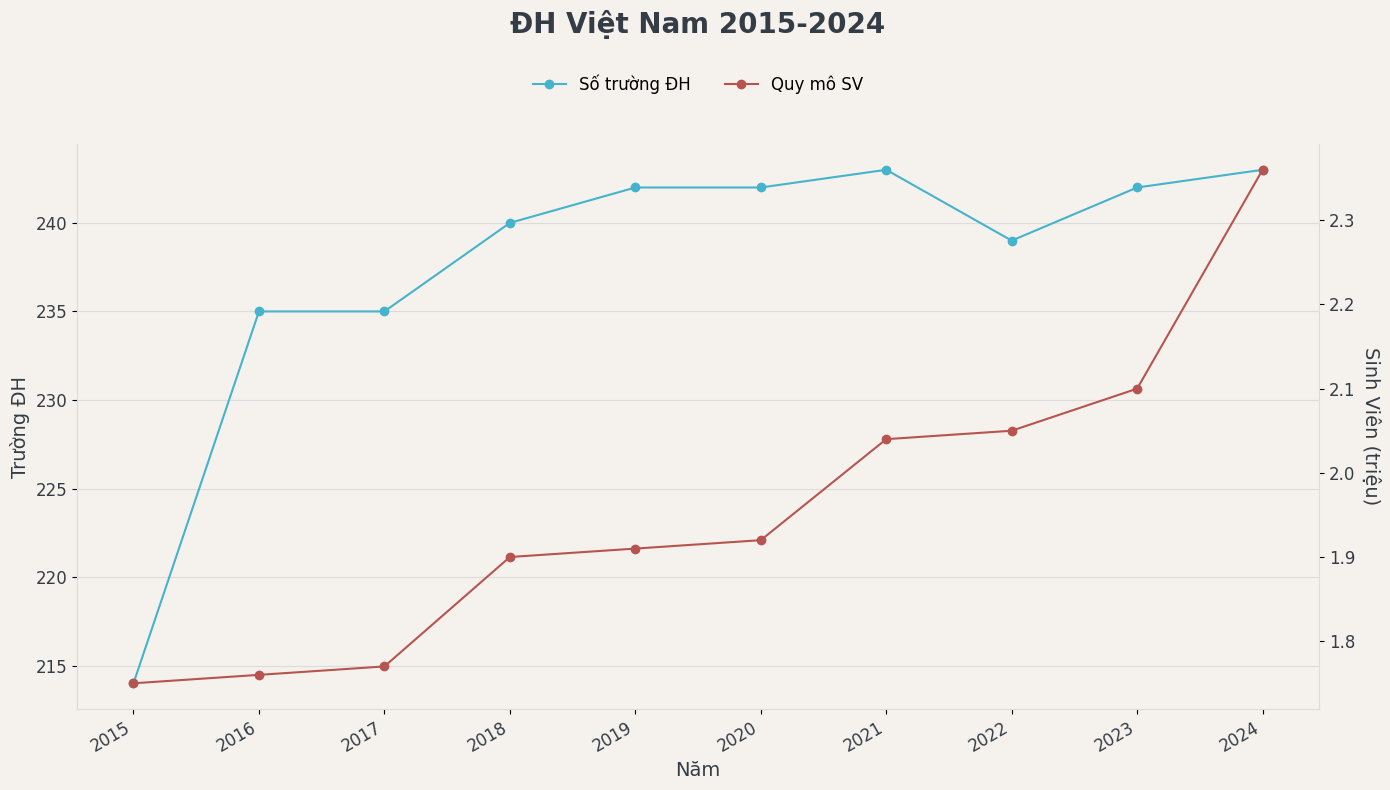
\includegraphics[width=\textwidth]{image/dh_viet_nam_2015_2024.png}
    \caption{越南高等教育办学机构数量与学生规模发展情况(2015-2024年)}
    \label{fig:so_truong_quy_mo_sv}
\end{figure}

分析图\ref{fig:so_truong_quy_mo_sv}显示了两种同步但速度不同的增长趋势。
\begin{itemize}
    \item \textbf{关于网络(蓝色线):} 高等教育机构数量呈现稳定而坚实的增长趋势,从2015年的215所增至2024年的243所。这一增长虽然不算突变,但反映了政府在拓展办学机构网络方面的一贯政策,包括成立新大学和升级专科学校,旨在为全国民众提供多样化的学习机会。
    \item \textbf{关于学生规模(红色线):} 与学校数量的平稳增长形成对比的是,学生规模呈现出异常强劲的爆炸性增长。在经历了2015年至2021年的相对稳定期后,学生规模在最后三年(2022-2024)内从约205万猛增至超过\textbf{235万学生}。这一飞跃不仅体现了高等教育日益增长的吸引力,也表明该体系正承受着为前所未有的大量学生提供培养需求的巨大压力。
\end{itemize}

这一增长正逐步使越南更接近到2030年实现\textbf{每万人口260名大学生}的国家战略目标\footcite{sggp_en_3million_2030}。此外,它还体现在重要的国际指标——高等教育毛入学率(GER)上。世界银行和联合国教科文组织的数据显示,越南的毛入学率已从2000年的仅10.3\%飙升至2018年的28.6\%,并于\textbf{2022年达到创纪录的42.22\%}\footcite{worldbank_humancapital_2022}。这是一项值得称道的成就,显示了教育大众化政策的成功。

\subsubsection{改善投入资源质量}
在扩大规模的同时,该体系的投入资源质量也取得了显著改善,显示了在提升内在能力方面的有目的的投资。
\begin{itemize}
    \item \textbf{师资队伍质量:} 拥有研究生学历(硕士或博士)的大学教师比例几乎翻了一番,从2007年的47\%增至\textbf{2020年达到85\%}\footcite{worldbank_p178112}。对提升师资队伍水平的投资是一个基础性因素,有望直接转化为教学和研究质量。
    \item \textbf{科学研究能力:} 提升教师水平的成就已产生具体影响。越南人均在国际权威期刊上可引用的科学文献数量,在十年间(2010-2020)\textbf{增长了三倍}\footcite{worldbank_improvingperformance_2020}。这表明该体系的研究能力取得了飞跃式进展,正逐步与国际科学界接轨。
\end{itemize}

上述数字和图表描绘了一幅关于悖论第一面的乐观画面:一个正在强劲发展、在网络、学生规模乃至投入资源质量等各方面都在扩张的高等教育体系。这些是不可否认的成就,为一个现代化和国际化的高等教育体系奠定了坚实的基础。然而,这幅画面只是一个更为复杂的悖论的一半。当我们将这些关于"量"的成就与关于产出质量和体系效率的指标进行对比时,一个充满挑战和警示的另一面故事开始显现。悖论的第二面将在下一部分深入分析。



% het goi 1


\subsection{悖论的第二面:质量的潜在危机与不匹配}
\label{subsec:ve_thu_hai_nghich_ly}

与规模和投入资源令人印象深刻的增长图景相反的是,关于产出质量和体系可持续性的 alarming signals。如果说悖论的第一面是一曲增长数字的交响乐,那么第二面则是一个残酷的现实,体现在培养规模与满足劳动力市场能力之间的分化。图\ref{fig:nghich_ly_quy_mo_chat_luong}清晰地将这一悖论可视化。

\begin{figure}[h!]
    \centering
    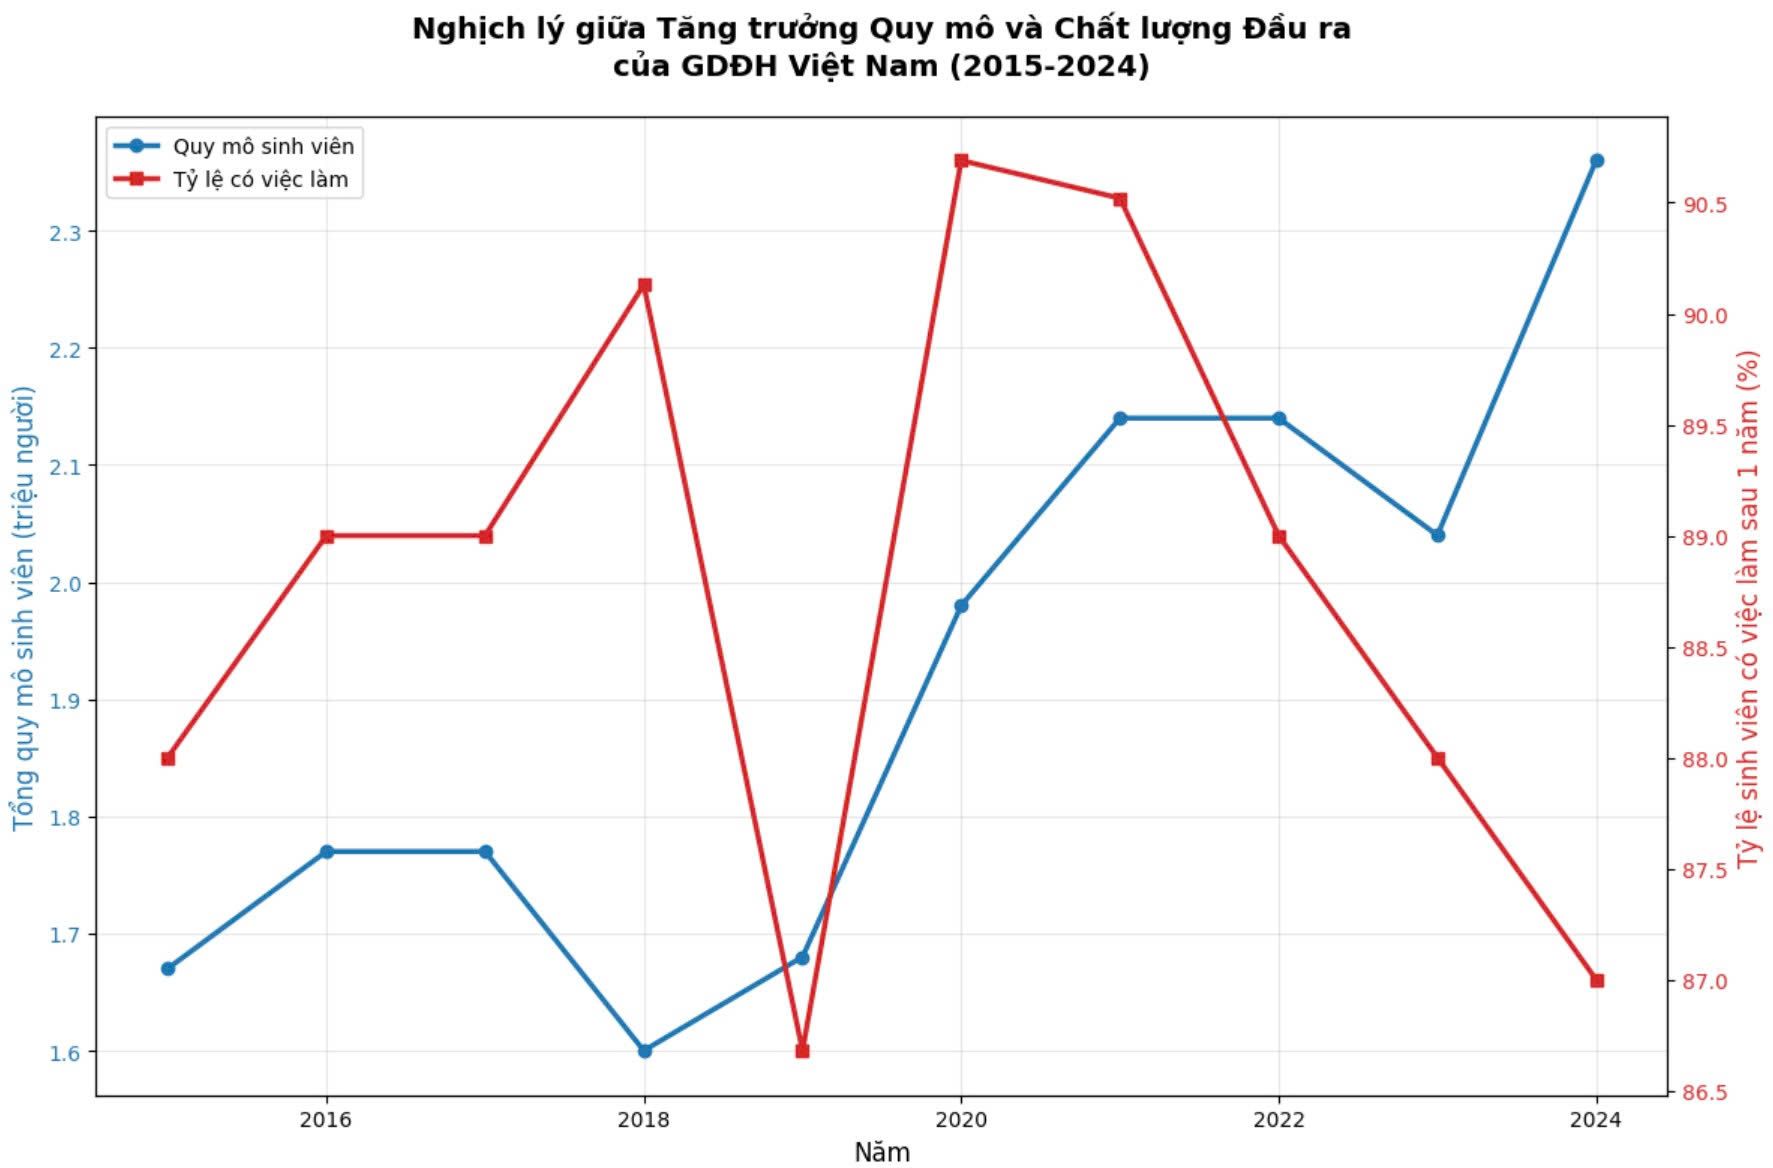
\includegraphics[width=\textwidth]{image/nghich_ly_tang_truong_quy_mo_chat_luong.jpg}
    \caption{越南高等教育规模增长与产出质量之间的悖论(2015-2024年)}
    \label{fig:nghich_ly_quy_mo_chat_luong}
    \vspace{0.2cm}
    \footnotesize{\textit{来源:综合整理自教育培训部数据及相关报告。}}
\end{figure}

\subsubsection{剖析"量"与"质"的分化}

图\ref{fig:nghich_ly_quy_mo_chat_luong}将两个重要指标置于同一坐标系中:学生总规模(左纵轴,蓝色线)和毕业一年后就业率(右纵轴,红色线)。理论上,在一个可持续发展的体系中,这两条线应呈正相关或至少保持稳定。然而,实际数据显示出一种令人担忧的分化(divergence):
\begin{itemize}
    \item \textbf{规模线(蓝色)}呈现出持续增长,特别是从2020年不到200万学生猛增至2024年超过230万学生。这再次证实了该体系面临的扩大规模的压力。
    \item \textbf{质量线(红色)}则呈现出完全相反的趋势。在2019-2020年左右达到峰值(超过90%)后,学生就业率出现了惊人的急剧下降,到2024年降至仅约87%。
\end{itemize}
这种分化正是发展悖论的"核心":当体系在规模上日益"膨胀"时,其最核心的价值——帮助学习者获得就业并为社会做贡献的能力——却在下降。这提出了一个紧迫的问题:难道对数量的追求已经严重损害了质量?

\subsubsection{来自劳动力市场的证据:失业、技能差距与不平等}

图表中"质量"线的下降趋势并非感性判断,而是由一系列来自劳动力市场和社會學分析的確鑿數據所證實。

\paragraph{失业与学非所用。} 劳动荣军与社会部的报告多次警示本科毕业生失业率高企,\textbf{2017年高达23.7万人},2018年仍有\textbf{22.55万人},约占全国失业总人数的20\%\footcite{vietnamnews_unemployed_2017}。这一数字,加上估计约有\textbf{60\%的毕业生从事与专业不符的工作},是因培养与需求脱节而造成社会和个人资源浪费的明显证据\footcite{britishcouncil_grad_employability_2021}。

\paragraph{技能差距。} 上述状况的深层原因在于严重的"技能差距"。英国文化协会的一项全面调查指出了一个令人担忧的现实:\textbf{73\%}的越南企业在招聘具备领导和管理技能的人才时遇到困难;\textbf{68\%}在寻找具备足够专业技能的员工时遇到困难;\textbf{54\%}表示缺乏具备必要社交情感技能的人才\footcite{britishcouncil_skills_gap_2021}。世界银行的报告也强调,近\textbf{80\%}的制造业公司在招聘熟练工人时遇到困难\footcite{worldbank_p178112}。这表明培养方案并未能为学生充分装备经济真正需要的技能。

\paragraph{机会不均与财务负担。} 除了质量问题,发展悖论还体现在不平等方面。尽管越南高等教育的个人回报率位居世界最高之列(年均超过15\%)\footcite{worldbank_improvingperformance_2020},但这一利益并未得到公平分配。数据显示,高达\textbf{80\%来自收入最高20\%家庭的青年}已经或正在接受大学教育,而这一比例在两个最低收入组中仅占学生总数的10\%\footcite{worldbank_p178112}。由于成本负担日益转向家庭(占公立学校总收入的\textbf{77\%})以及学生贷款项目的缩减,这种不平等正面临着加剧的风险\footcite{worldbank_p178112}。

总之,悖论的第二面展示了一幅充满挑战的图景:一个尽管在规模和资源上投入巨大,但其产出却未能满足市场要求,同时潜藏着社会不平等风险的体系。清晰地认识这一悖论的两个方面,是能够准确"诊断"系统性"病症"的先决步骤,这一任务将在本章的后续部分进行。


% het goi 2



\section{塑造质量的主体与制度框架}
\label{sec:khung_the_che}

从已证明的"发展悖论"图景中,一个核心问题被提出:体系中的哪些力量和主体,以何种方式行动,从而造成了这一现状?要回答这个问题,首先需要识别主要的利益相关者,并分析主导该体系"游戏规则"的制度框架。

\subsection{高等教育质量保障生态系统中的利益相关者图}

越南高等教育质量保障体系是一个复杂的生态系统,有众多利益相关者参与其中,每一方都扮演着不同的角色、拥有不同的利益和影响力。图\ref{fig:so_do_he_thong_dbcl}提供了该生态系统中主要主体的概览。

\begin{figure}[h!]
    \centering
    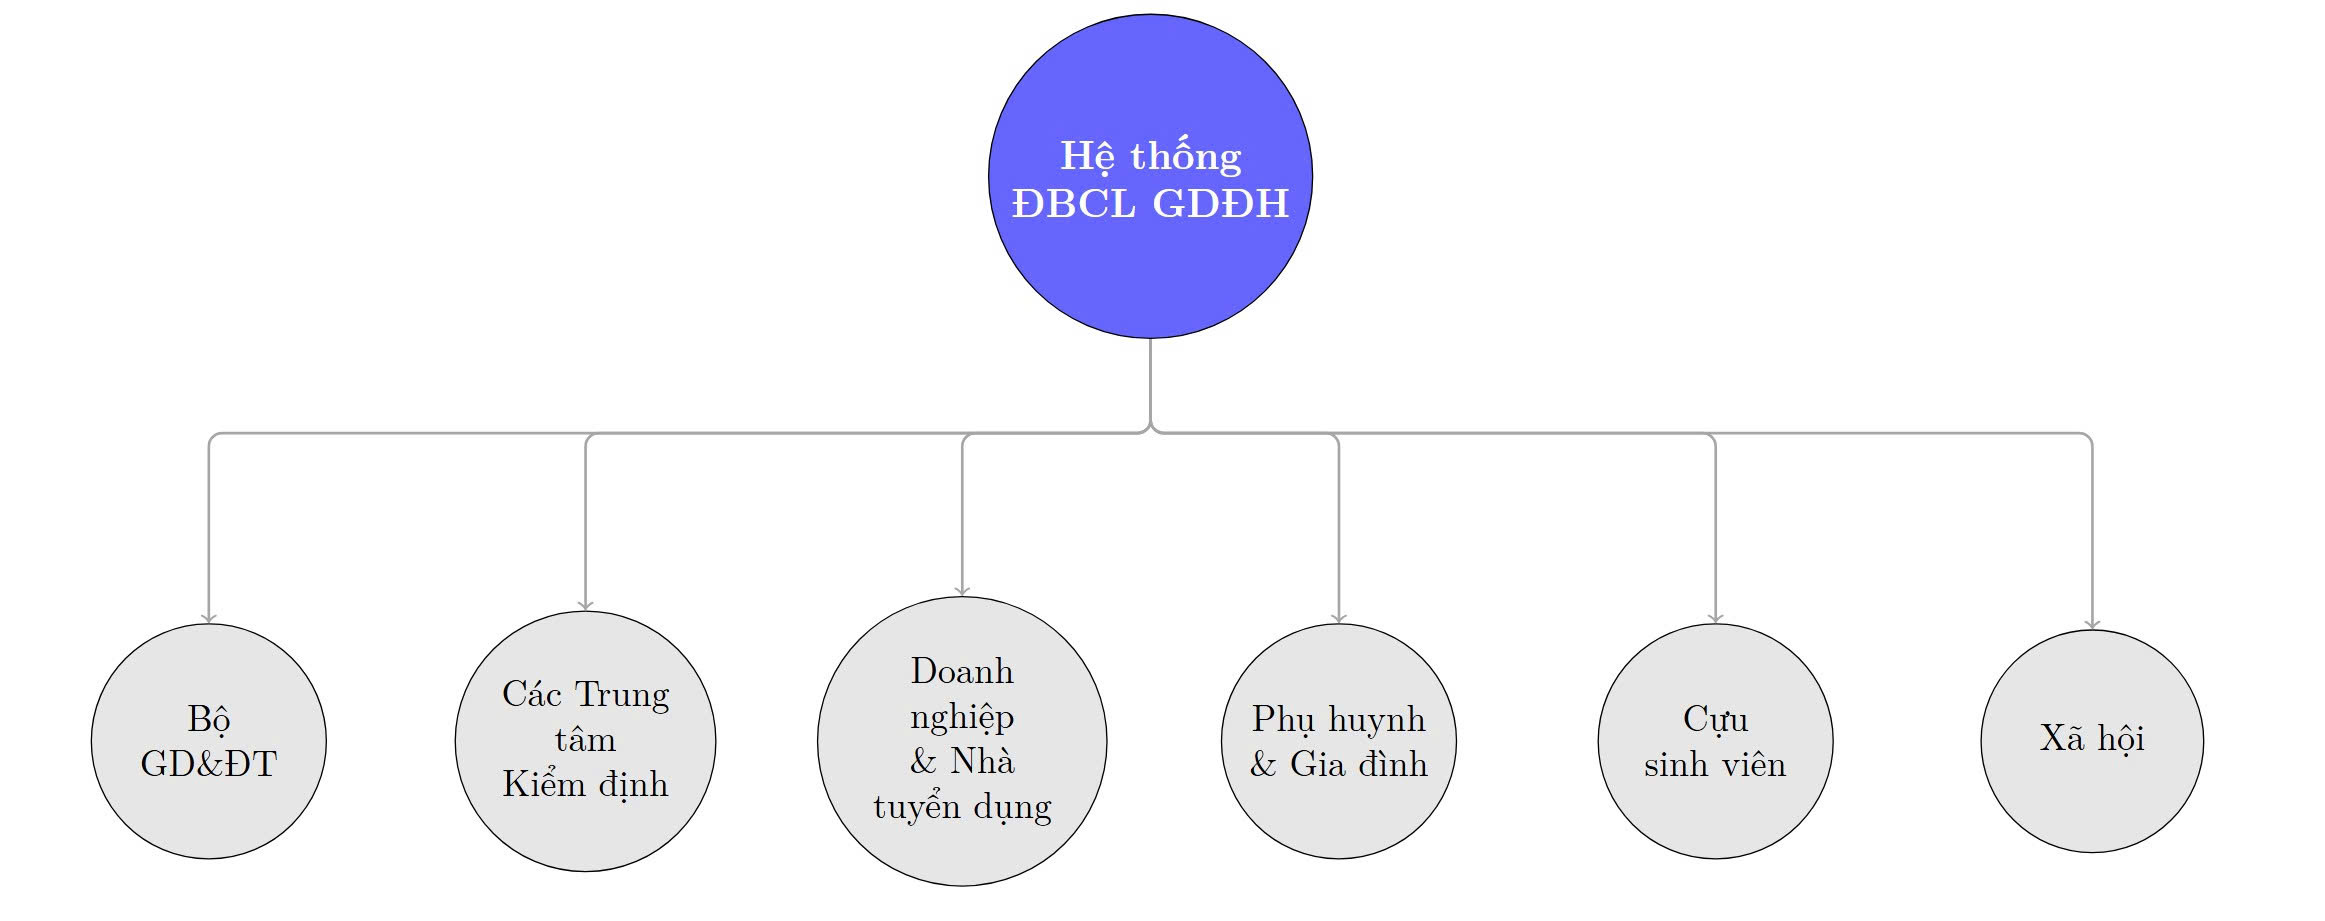
\includegraphics[width=\textwidth]{image/he_thong_dbcl_gddh.jpg}
    \caption{越南高等教育质量保障体系中的主要利益相关者图}
    \label{fig:so_do_he_thong_dbcl}
\end{figure}

上图可分为两大主要群体:
\begin{enumerate}
    \item \textbf{管理与执行群体(左侧与中心):} 包括国家机构和被直接授权的组织,扮演着制定政策和执行认证活动的角色。该群体包括\textbf{教育培训部}和各\textbf{认证中心}。
    \item \textbf{监督与受益群体(右侧):} 包括社会中的各个主体,他们是高等教育"产品"的直接使用者,并为质量提供重要的反馈。该群体包括\textbf{企业与雇主}、\textbf{家长与家庭}、\textbf{校友},以及更广泛的整个\textbf{社会}。
\end{enumerate}
分析这些主体,特别是制定"游戏规则"的群体之间的角色和关系,将阐明正在塑造越南质量保障现状的动因和压力。

\subsection{教育培训部:游戏规则的制定者与合规性压力}
\label{subsec:vai_tro_moet}

在越南的质量保障生态系统中,教育培训部扮演着核心权力主体的角色,负责构建和协调整个体系。从委托代理理论的视角来看,教育培训部是最高的"委托人",将培养和保障质量的任务委托给各大学(代理人)\footcite{Kivisto2008}。同时,根据新制度主义理论,该部是产生最强大"强制性压力"的源头,迫使各大学遵守一个共同的法规框架,以获得合法性并维持运作\footcite{MeyerPowell2020}。

这种引领作用通过颁布一系列法规文件得以清晰体现,其核心精神由关于"根本性、全面性教育与培训革新"的第29号决议所指导\footcite{nghi_quyet_29_2013}。该决议明确提出了"增强教育培训机构的自主权和社会责任"以及建立一个"独立的认证体系"的要求。正是这些战略性导向,构建了法律走廊,推动各大学逐步与区域及国际标准接轨。

然而,这种集中的垂直管理机制,虽然对于确保统一性是必要的,但也正是导致许多教育机构形成一种\textbf{"合规文化"}而非\textbf{"改进文化"}\footcite{pham2021governance}。各大学,特别是严重依赖国家预算的公立大学,倾向于优先开展旨在满足该部的报告要求和认证标准的活动,有时会轻视来自内部的实质性改进。因此,教育培训部既扮演着"游戏规则"制定者的角色,又是最高监督者,创造了一个合规性通常被置于创新之上的制度环境。

\subsection{质量认证中心:政策执行与独立性问题}
\label{subsec:vai_tro_trungtamkd}

如果说教育培训部是"委托人",那么各教育质量认证中心则扮演着重要的"代理人"角色,其任务是具体化和执行认证政策。这些中心体系的发展,是越南质量保障活动制度化努力的证明。截至2024年初,全国共有7家获准运营的教育质量认证中心,包括公立和私立单位\footcite{tuoitre_kdcl_stats_2024}。

该体系已积极运作,在执行国家质量政策方面扮演着重要的"延伸手臂"角色。截至2023年底,这些中心已对全国\textbf{1855个培养项目}和\textbf{187所教育机构}进行了认证和承认\footcite{tuoitre_kdcl_stats_2024}。2021年两家私立中心的成立,也标志着朝着社会化、评估单位多样化方向迈出了新的一步。

然而,学术界和管理层提出的一个重要问题是这些中心的\textbf{实质性独立性}。尽管是以独立法人身份成立,但7家中心中有5家仍是大型大学或协会的下属单位,并且所有中心都在教育培训部的严密监督下运作。这种"既是主管单位,又是被认证对象"的关系,可能会引起人们对评估结果绝对客观性的怀疑\footcite{giaoducnet_kdcl_list_2023}。更重要的是,它有可能会进一步强化大学的合规压力。许多学校并未将认证中心视为共同改进的伙伴,而是仍然抱着应付上级"检查"的心态。这种复杂的关系将在后续章节中,在审视质量文化和体系协调等挑战时进行更深入的分析。


% het goi 3




\section{基于V-AQA模型的现状分析}
\label{sec:phan_tich_vqa}

在确定了主要主体的角色和体系的"游戏规则"之后,本章将运用V-AQA模型的五个要素,系统地"解剖"越南高等教育质量保障体系所面临的核心挑战。分析将从问题的源头——领导能力和组织文化——这两个具有紧密因果关系并塑造校内所有质量活动的要素开始。

\subsection{要素一:领导与治理的挑战——自主与合规之间}
\label{subsec:thach_thuc_lanhdao}

\textbf{领导与治理}要素是整个质量保障体系的发起、导向和提供能量的源泉。它体现在高层领导团队(校董会、校领导班子)在战略上引领学校实现质量目标的愿景、承诺和能力。然而,在越南,这一领导角色正处于两难境地,被困在推动自主的政策和仍然带有浓厚合规性的管理实践之间。

\subsubsection{自主政策与管理实践的矛盾}
尽管大学自主的主张已在修订后的《高等教育法》中制度化,但在实际推行中仍存在诸多障碍。顶尖专家已指出规定与实践之间的严重不匹配。根据顶尖高等教育政策专家之一\textbf{范氏丽博士}的分析,现行大学自主的法律框架如同"一件遮不住身体的紧身衣"\footcite{lypham_aosat_2024}。她论证道,"主管部门"的概念仍然是一个巨大的障碍,这种理解与国际惯例相去甚远,削弱了自主的本质。公立大学倾向于只向管理层"报告",而不是真正地对社会就培养质量负责,这使得问责制变得形式化。

同样,前高等教育司副司长\textbf{黎曰劝博士}也提出了一个坦率的看法:"不废除主管部门机制,就别急着转向自主"\footcite{khuyen_bochuquan_2022}。他分析称,只要主管部门还存在并有权干预人事和财务决策,校董会的实质性自主权就会受到限制。届时,学校领导者的角色很难摆脱行政命令执行者的地位,而不是成为一个真正的战略管理者。

\subsubsection{后果:领导层优先级的转移}
这种情况的直接后果是,领导团队在质量方面的战略管理能力未能得到充分发挥。许多管理者不得不将大部分时间和精力用于处理行政程序和满足上级要求,而不是能够专注于制定长期决策,如建设质量文化、推动创新或建立战略联盟。他们的重心从"如何实质性、可持续地提升质量?"这一问题,转移到更短期的"如何完成报告并通过认证评估?"这一问题上。这种优先级的转变是一个无形但极其强大的障碍,它抑制了来自基层的创新努力,并直接催生了下文将分析的应付式质量文化。

\subsection{要素二:质量文化的挑战——从被动合规到主动改进}
\label{subsec:thach_thuc_vanhoa}

如果说领导与治理要素是质量保障体系的"大脑",那么\textbf{质量文化}就是其"灵魂",是决定质量流程是得到实质性执行还是仅为形式应付的关键因素。哈维和斯坦塞克(2008)将质量文化定义为一个共享的价值观和信念集合,组织中的每个成员都自觉地致力于持续改进\footcite{HarveyStensaker2008}。然而,实践证据表明,这是越南高等教育中最重大且固有的挑战之一,是上述带有浓厚合规性管理模式的直接后果。

\subsubsection{"反应型质量文化"的定性}
一项关于越南大学质量文化的深入研究,将这一特征定性为一种\textbf{"反应型质量文化"}\footcite{vjol_reactiveculture_2021}。在此层次上,组织仅在出现问题或有外部压力(例如:认证评估)时才关注质量,而不是主动寻找改进机会。质量保障活动通常只在认证周期临近时才被大力推动,并在学校获得证书后趋于"沉寂"。这是质量保障研究中常称的"季节性活动"或"认证风暴"现象。

从新制度主义理论的角度看,这是"脱钩"现象的典型表现,即组织形式上采纳所要求的结构和流程以获得合法性,而内部核心活动(教学、学习、研究)却无实质性改变\footcite{MeyerRowan1977}。这种文化的直接后果是学术团队的被动参与。本应是改进过程主体的教师和员工,却常常将质量保障活动视为一种行政负担,一种教学专业之外的"额外工作"\footcite{iosr_passiveparticipation_2021}。

\subsubsection{通过社会信任的波动表现出来}
内在质量文化的脆弱性必然会通过社会的信任度反映出来,而考生和家庭的入学决定是一个敏感指标。图\ref{fig:ty_le_nhap_hoc}显示了2015-2024年间考生确认入学比例的显著波动。

\begin{figure}[h!]
    \centering
    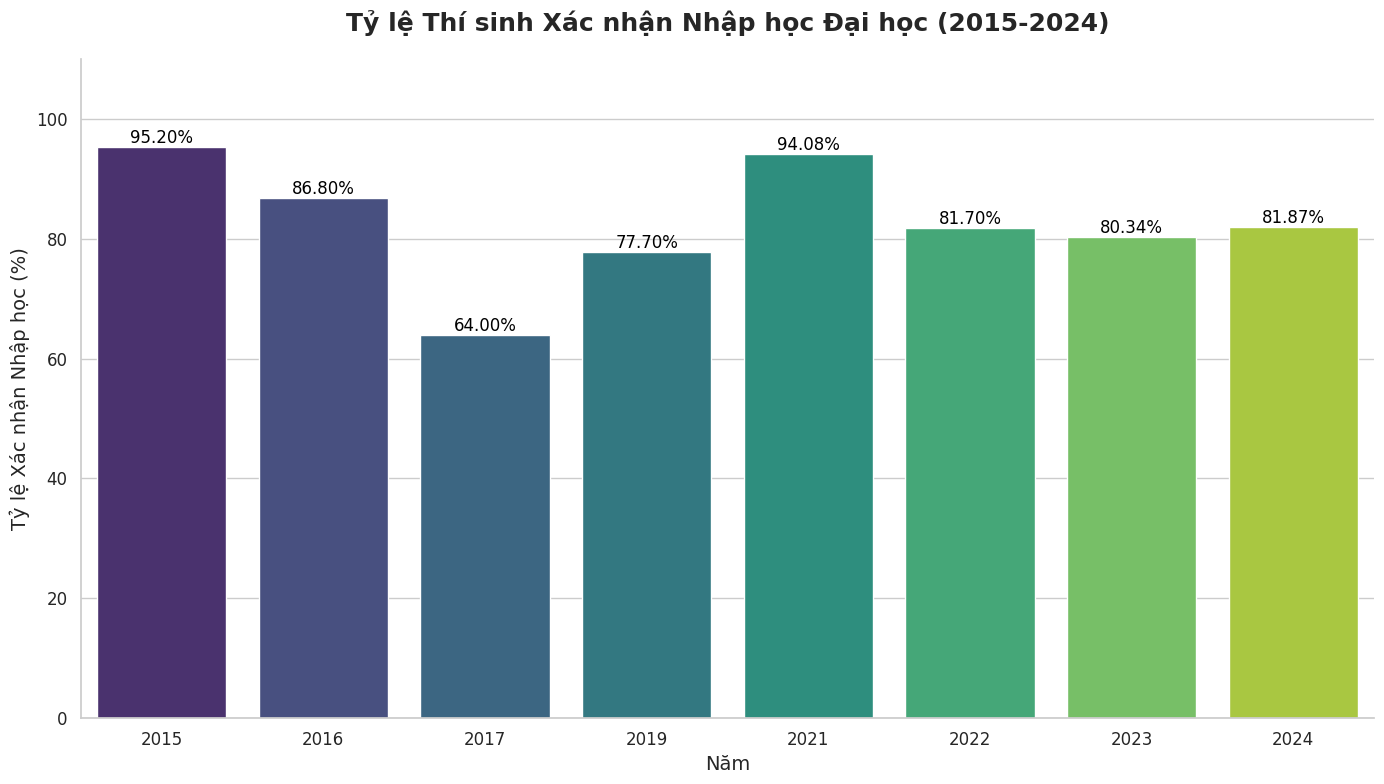
\includegraphics[width=\textwidth]{image/ty_le_nhap_hoc_2015-2024.png}
    \caption{大学新生确认入学比例(2015-2024年)}
    \label{fig:ty_le_nhap_hoc}
    \vspace{0.2cm}
    \footnotesize{\textit{来源:综合整理自教育培训部历年招生数据。}}
\end{figure}

图表并未呈现稳定的增长趋势,而是显示出剧烈波动。特别是,从2016年的86.8\%急剧下降到\textbf{2017年的仅64\%},是一个令人警醒的信号。这种突降不能仅用招生规定的变化来解释,更可以被解读为当时社会对大学文凭价值和质量的一次"信任危机",此前媒体已长期广泛报道本科生失业问题。

近年来该比例的回升并维持在较高水平(80%以上),显示了整个体系的改进努力,尤其是在修订后的《高等教育法》生效之后。然而,正是这种波动表明,利益相关者的信任仍然脆弱,越南高等教育的感知质量尚未真正稳固。一个实质性的、来自内部的质量文化,需要创造一个稳定可靠的承诺,而不是像这样充满波动且依赖外部因素的结果。

\subsubsection{打破惰性的努力:促进机制的案例研究}
尽管合规文化仍然普遍,但一些教育机构已开始率先采用具体的治理机制来打破这种惰性。一个典型案例是\textbf{胡志明市技术大学}。自2022年起,该校推行了一项具有杠杆作用的政策:学生必须完成关于教师教学活动的在线调查,才能查看该课程的期末考试成绩\footcite{hutech_khao_sat_2022}。
这项政策创造了一个积极而强大的反馈循环。学生完成调查问卷的比例达到非常高的平均水平,提供了一个巨大而全面的反馈数据源。面对这些数据,教师被迫倾听并参与到改进过程中。结果显示,许多教师已主动调整方法、更新课件幻灯片并补充实践案例。这个案例生动地说明,质量文化并非一个抽象概念,而是可以通过足够强大的具体治理机制来影响和塑造,从而从被动参与转变为主动调整。


% het goi 4



\subsection{要素三:利益相关者参与的挑战——"象牙塔"与市场之间的鸿沟}
\label{subsec:thach_thuc_lienquan}

\textbf{利益相关者参与}要素是"质量为谁服务?"这一理念的实现。它要求教育机构从封闭、内向的管理模式转向开放模式,在此模式中,社会主体,特别是学生和雇主的呼声和需求,被实质性地倾听并整合到所有改进周期中。然而,实践证据表明,这正是系统性的薄弱环节之一,是导致本章开头所分析的"发展悖论"和"技能差距"的直接原因。

\subsubsection{有限且形式化参与的表现}
通过认证报告和学术研究记录到的最普遍的现状是"缺乏从雇主、校友那里系统性、持续性地收集反馈的机制;企业对培养方案设计和审查过程的参与有限且缺乏连续性"\footcite{vnujs_er_2018}。互动活动(如果有的话)通常是形式化、零散和被动的。它们通常作为一种"应付"活动来进行,以完善认证档案——例如,合作备忘录被大张旗鼓地签署,却没有具体的实施计划;或者调查问卷仅为存档作为证据而进行——而不是真正利用收集到的数据来战略性地改进培养方案\footcite{vje_aun_implementation_2019}。

校企联系薄弱,通过世界银行令人警醒的统计数据得以体现:\textbf{"不到3\%的企业声称在产品创新方面与大学或研究机构合作"}\footcite{worldbank_improvingperformance_2020}。这一数字不仅反映了研发合作的缺失,更暗示了一个更深层次的问题:缺乏一种战略伙伴关系,让双方共同参与培养方案的设计、实施和评估。其后果是,培养方案通常只反映教师纯粹的学术观点,这是"象牙塔"思维的遗留物,而缺乏来自行业的实践视角。这创造了一种无法满足其最终"客户"——劳动力市场——要求的教育产品。

\subsubsection{通过阿恩斯坦参与阶梯分析参与程度}
为了更深入地理解形式化参与的程度,可以运用雪莉·阿恩斯坦的"公民参与阶梯"模型\footcite{Arnstein1969}。尽管该模型诞生于城市规划背景下,但它为评估教育中利益相关者实质性参与的程度提供了一个有效的分析框架。阿恩斯坦将参与分为八个梯级,归纳为三个主要层次:
\begin{enumerate}
    \item \textbf{无参与 (Non-participation):} 包括"操纵"和"治疗"两个梯级,其真实目的是"教育"或"治愈"参与者。
    \item \textbf{形式化参与 (Degrees of Tokenism):} 包括"告知"、"咨询"和"安抚"三个梯级。在此层次上,利益相关者的声音被倾听,但他们没有真正的权力来确保其观点会被采纳并据此行动。
    \item \textbf{公民权力 (Degrees of Citizen Power):} 包括"伙伴关系"、"授权"和"公民控制"三个梯级,在此层次上,利益相关者在决策中拥有真正的权力。
\end{enumerate}
对照越南高等教育的现状,可以看出大多数校企"合作"活动被困在了\textbf{形式化参与}的层次。诸如发送研讨会邀请函、发送培养方案调查问卷等活动仅停留在"告知"和"咨询"的梯级。利益相关者可以提出意见,但没有明确的机制来确保这些意见会转化为课程的具体改变。缺乏"伙伴关系"层级的模式,是缩小技能差距的最大障碍。

\subsection{要素五:合作与协调的挑战——被孤立的"孤岛"}
\label{subsec:thach_thuc_hoptac}

如果说利益相关者的参与是改进过程的"输入",那么\textbf{合作与协调}的能力就是处理和传播这些价值的"机器"。然而,越南高等教育的现状表明,这是一种薄弱的能力,在组织内部合作、大学之间合作以及与外部利益相关者合作这三个层面上都表现明显。这三个层面同步的薄弱,已将许多大学变成了被孤立的"孤岛",降低了质量改进努力的成效。

\subsubsection{第一层面:内部合作——组织内的碎片化}
合作的挑战通常始于每所大学的内部。"各自为政"、碎片化以及缺乏各院、处、室之间同步协调的机制是一种普遍现象。教务处、质量保障处、科技处、学生工作处等职能部门以及各专业院系通常独立运作,追求各自的目标,而缺乏与学校整体质量战略的联系。这种碎片化,也称"筒仓思维",导致了职能重叠、资源浪费和政策不一致。
最明显的后果是关于学生、培养方案、就业率的数据碎片化、不一致且难以获取——这个问题将在第八部分深入分析。同样,一个培养方案在设计时缺乏与其他院系和支持单位的广泛协商,也反映了"部门本位"思维,即每个院系将培养方案视为自己的"私有财产",而非全校的共同产品。

\subsubsection{第二层面:校际合作——竞争压倒合作}
在体系层面,越南高等教育环境本质上仍然是一个在招生、排名和有限资源方面竞争激烈的环境。这无形中为开放地分享经验和相互学习设置了障碍。诸如质量标杆比对或校际同行评审等活动,尽管受到鼓励,但通常仅形式化地进行,未能深入。
竞争性的"零和"思维(即一方的收益等于另一方的损失)使得各校倾向于将"最佳实践"保留给自己,并将兄弟院校视为对手,而不是将它们视为共同发展的教育生态系统中的合作伙伴。缺乏一个能让各校公开分享成功与失败以共同学习的实质性合作网络,减缓了整个体系整体质量水平的提升进程。

\subsubsection{第三层面:与社会合作——松散的联系}
这是合作最薄弱且记录最明显的一个层面。如前所述,缺乏来自利益相关者反馈的核心原因在于"封闭式管理文化"和建立战略伙伴关系能力的缺失。由于未能设计出互利共赢的双边合作项目,越南大学将自己与来自社会的重要知识和财政资源隔离开来。
正是为了打破这堵"墙",像\textbf{行业咨询委员会}这样的先锋模式应运而生。典型的是在越南皇家墨尔本理工大学、胡志明市国家大学下属的百科大学(在BUILD-IT项目的支持下),以及近期的VinUni大学等高校有效实施的模式。这些委员会不仅停留在咨询层面,还直接参与塑造战略和改进培养方案,创造了一个实质性的对话与合作渠道\footcite{rmit_iab_2023}。

% het goi 5


\subsection{打破象牙塔壁垒的先锋模型}
\label{subsec:mo_hinh_tien_phong}

尽管校企联系不足的普遍现状是一个系统性挑战,但一些先锋教育单位已经并正在努力构建实质性的合作模式,超越了形式化的活动。深入分析这些案例研究,不仅提供了关于"最佳实践"的典型范例,也为可持续地解决"技能差距"问题启示了潜在的方向。这些模型体现了一种思维的转变:从"求-给"关系转变为"战略伙伴共同创造价值"的关系。

\subsubsection{行业咨询委员会模型:从咨询到共同创造}
这是在先进大学中应用最普遍且最成功的模型,其作用是将行业的声音带入学术决策过程的中心。一个有效的行业咨询委员会不是一个形式化的咨询班子,而是一个活跃的实体,深入参与培养方案的生命周期。

\paragraph{BUILD-IT联盟与工科院校群的案例研究。} 在美国国际开发署的技术和资金支持下,由亚利桑那州立大学牵头的BUILD-IT联盟已成为在越南推行国际标准行业咨询委员会的典范。在胡志明市国家大学下属的百科大学、岘港大学和芹苴大学等顶尖工科院校,工科领域的行业咨询委员会已产生显著影响:
\begin{itemize}
    \item \textbf{共同创造培养方案:} 来自英特尔、罗克韦尔自动化、eSilicon等全球科技集团的行业咨询委员会成员,直接参与审查和提出建议,以调整预期学习成果。他们帮助将关于"工业4.0"、"芯片设计"或"自动化"的知识实质性地引入课程,确保这些课程能够满足像ABET这样严格的国际认证标准。这相比仅仅发送问卷征求意见,是一个巨大的进步\footcite{buildit_iab_impact}。
    \item \textbf{赞助与能力建设:} 企业不仅"提意见",还"投资"。许多公司赞助了设备,在校园内建立了现代化的实验室,帮助学生接触到学校难以凭自身经费装备的技术。
    \item \textbf{为学生搭建桥梁:} 行业咨询委员会中的企业承诺共同指导学生的毕业设计项目,为学生提供解决行业真实问题的机会。他们也是高质量实习岗位和工厂参观项目的提供者,帮助学生尽早构想专业工作环境。
\end{itemize}
BUILD-IT的模型之所以成功,是因为它建立在双方互利的基础上:学校获得了高质量且获国际认证的培养方案,而企业则获得了根据自身需求"量身定做"的未来人力资源。

\paragraph{越南皇家墨尔本理工大学的案例研究。} 作为一所国际大学,皇家墨尔本理工大学已将全球标准的行业咨询委员会模型引入越南并系统地运作。该校每个专业都有一个独立的咨询委员会,成员包括来自毕马威、联合利华、汇丰银行等行业领军企业的高层领导。
\begin{itemize}
    \item \textbf{定期与专业的运作机制:} 这些委员会每年至少定期召开两次会议,议程明确:审查行业新趋势,重新评估课程的预期学习成果,并为课程结构提出必要的修改建议。这种咨询确保了课程始终与市场的最新趋势保持同步,从"数字经济"到"商业数据分析"\footcite{rmit_iab_2023}。
    \item \textbf{双向影响:} 这种关系为双方都带来了利益。皇家墨尔本理工大学获得了契合需求的培养方案,而企业则有机会接触到高质量的人力资源,同时提升其在学生群体中的雇主品牌。
\end{itemize}

\paragraph{VinUni大学的案例研究。} VinUni大学自建立之初就秉持与企业紧密结合的理念,将来自Vingroup集团及其合作伙伴的专家的角色深度融入培养过程。VinUni的模型超越了传统的行业咨询委员会,致力于打造一个"企业内学习"的生态系统。
\begin{itemize}
    \item \textbf{在教学和研究中融合:} 许多Vingroup的高层领导直接参与课程的授课或专题报告。教师和学生的研究课题也常常源于各成员公司的实际问题。
    \item \textbf{基于大型项目的学习:} 学生有机会参与到VinFast(开发自动驾驶汽车)、VinAI(研究人工智能)、VinBrain(开发医疗解决方案)等成员公司的实际项目中,创造了一个独特且大规模的基于项目的学习环境\footcite{vinuni_industry_collaboration_2023}。该模型有助于消除理论与实践之间的鸿沟,这是越南高等教育的一个固有挑战。
\end{itemize}

\subsubsection{其他深度合作模型}
除了行业咨询委员会,更深层次的合作形式也已开始出现,显示出调动社会资源的巨大潜力。

\paragraph{公私合作伙伴关系模型在研究与培养中的应用。} 一个突出的例子是胡志明市国家大学的战略。该校不只依赖国家预算,而是主动构建公私合作伙伴关系项目,在2016-2021年间从企业动员了超过\textbf{4000亿越南盾},投资于超过\textbf{230个研发项目}、重点实验室和研究生培养项目\footcite{vnuhcm_ppp_2022}。该模型不仅解决了经费问题,还确保了研究和培养活动始终与企业的实际问题紧密相连。

\paragraph{企业学期模型。} 一些学校,如FPT大学,已率先采用"在岗培训"模型,这是一种校企合作教育的形式,其中三年级学生必须在合作企业全职工作一个学期(4到8个月)。在此期间,学生被视为正式员工,被分配真实的工作任务,并根据绩效进行评估。该模型帮助学生在校期间就积累实际工作经验,发展软技能并建立人际网络。这是对雇主常抱怨的"缺乏经验"和"缺乏技能"问题的直接解决方案。

\bigskip
上述案例研究,尽管并非全景,但生动地证明了打破"象牙塔壁垒"是完全可行的。它们表明,当有正确的战略、领导层的承诺以及一个互利共赢的合作机制时,越南的大学可以缩小与劳动力市场的差距。然而,这些外部联系的成效在很大程度上取决于校内流程的吸收和处理能力。下一部分将回到体系的"黑箱",分析这些内部流程。


% het goi 6 chuong 3



\subsection{要素四:内部流程的挑战(第一部分)——质量的"硬件}
\label{subsec:thach_thuc_quytringnoibo_hard}

如果说前面的要素关注的是方向、文化和互动,那么\textbf{内部流程}要素正是技术的"机器",是质量目标得以实现或失败的地方。对这些核心流程的分析,揭示了在设计教育"产品"及保障该产品产生的条件方面,存在系统性的薄弱环节。本部分将重点关注有形的"硬件"要素:培养方案和物质资源。

\subsubsection{培养方案的设计与审查:设计与实践的脱节}

培养方案的设计流程是起点,是决定整个教育过程质量的蓝图。然而,这恰恰是受到最多批评和最为薄弱的环节之一,是第二部分所证明的"技能差距"的直接原因。

\paragraph{预期学习成果的薄弱。} 最大的挑战在于构建预期学习成果。多项研究和认证报告指出了一个普遍的现状:"预期学习成果设计模糊,缺乏可衡量性,未能真实反映劳动力市场所需的能力"\footcite{vnujs_pam_2019}。许多培养方案的预期学习成果并非基于对利益相关者需求的深入分析而构建,而是"泛泛而谈,抄袭而来,没有企业的参与"\footcite{ijlter_elo_copy_2021}。这种情况是第五部分所分析的与企业合作和咨询机制薄弱的直接后果。

\paragraph{打破"建设性对齐"原则。} 确定预期学习成果的薄弱,导致了在应用基础教学原则——比格斯和邓的"建设性对齐"原则——方面的系统性失败\footcite{Biggs2011}。该原则认为,在一个高质量的培养方案中,三个组成部分之间必须有紧密和逻辑的对齐:\textbf{预期学习成果}(学生需要达到的目标)、\textbf{教与学活动}(帮助学生达到预期学习成果的活动),以及\textbf{评估活动}(衡量达到预期学习成果程度的方法)。
当预期学习成果写得模糊笼统时,就不可能为设计合适的教学活动和评估方法提供坚实的基础。教师会根据经验和现有知识进行教学,而考试则主要考察理论记忆能力,而不是衡量像批判性思维、解决问题或团队合作等复杂能力。这种对齐原则的打破,是解释为何越南学生虽然分数高,但在毕业时却缺乏实际技能的根本原因之一\footcite{csph_iqa_2023}。

\subsubsection{资源与物质设施:融入国际的薄弱基础}

一个培养方案即使设计得再好,如果没有资源和物质设施的保障条件,也无法有效运作。当越南许多大学努力接轨东盟大学网络等区域和国际标准时,这仍然是一个巨大的挑战。

\paragraph{设备的落后状况。} 许多报告指出了"设备、实验室落后;图书馆缺乏更新的国际学习资源;物质设施不满足按国际标准培养的要求"\footcite{vjes_challenges_aun_2020}。这种短缺在科学、技术、工程和医药等领域尤为严重,因为这些领域的学生需要在现代化的机器和设备上进行实践。当实验室不足或过于陈旧时,培养将偏重于空洞的理论,进一步加深了学校知识与实践要求之间的鸿沟。

\paragraph{信息通信技术基础设施的瓶颈。} 世界银行的报告指出了一个在数字化转型背景下日益严重的固有弱点:\textbf{"越南大学的信息通信技术基础设施仍然不发达"}\footcite{worldbank_improvingperformance_2020}。信息通信技术基础设施的薄弱不仅影响了实施现代教学方法(如混合式学习、翻转课堂)、获取数字学习资源和开展高质量研究的能力,还直接阻碍了构建集成的管理信息系统。这正是阻碍有效实施质量保障管理信息系统和高等教育管理信息系统的"硬件"障碍,这个问题将在下一部分深入分析。

\paragraph{系统性原因。} 物质设施的薄弱不仅仅是少数几所学校的故事,而是源于系统性的原因。首先是"公共投资预算有限",导致学校没有足够的资源进行同步投资和定期升级设备。此外,"官僚化的公共采购流程"和复杂性也是一个巨大障碍,即使学校获得了资金,也减缓了物质设施现代化的进程\footcite{vjes_challenges_aun_2020}。最后,缺乏一个关于物质设施发展的长期战略规划,也导致投资通常是零敲碎打、缺乏同步性,无法满足学校长期的可持续发展要求。

% het goi 7



\subsection{要素四:内部流程的挑战(第二部分)——体系的"阿喀琉斯之踵"}
\label{subsec:thach_thuc_quytringnoibo_achilles}

如果说培养方案的设计流程是起点,那么收集、分析和使用数据以进行评估和改进的流程,正是"神经系统",是一个能够自我调节和学习的质量保障体系的基础。然而,来自实践的证据和国际报告都指出,这恰恰是系统性且最严重的薄弱环节,被视为瘫痪越南绝大多数大学实质性质量改进努力的\textbf{"阿喀琉斯之踵"}\footcite{worldbank_improvingperformance_2020}。

\subsubsection{数据驱动治理薄弱的表现}
数据驱动治理能力薄弱体现在许多具体和系统性的表现上:
\begin{itemize}
    \item \textbf{评估方法不全面:} 认证报告和研究经常指出,"课程评估方法不全面,缺乏实证数据来衡量培养效果"\footcite{csph_iqa_2023}。学校通常只依赖于易于收集的数据,如学生分数、毕业率,而缺乏更深入的数据,如每个预期学习成果的达成度、毕业1-2年后从事对口工作的学生比例,或雇主对具体技能组合的满意度。
    
    \item \textbf{数据碎片化且不一致:} 这是一个"痼疾"。数据通常是碎片化的,分散在不同的处、室(教务处、学生工作处、科技处、质量保障中心等),格式各异,且互不联通。这种情况,部分是由于第五部分所分析的"筒仓思维"造成的,使得要汇总一幅关于某个培养方案或整个学校质量的全景图变得极其困难和耗时\footcite{aunsec_redesigningIQA_2022}。
    
    \item \textbf{缺乏集成的管理信息系统:} 在宏观层面,世界银行指出的最大障碍之一是"在国家层面同步和统一的高等教育管理信息系统仍未得到彻底部署"\footcite{worldbank_improvingperformance_2020}。缺乏一个有效的国家高等教育管理信息系统,其后果是各学校也缺乏动力和共同标准来系统地构建校级管理信息系统。
\end{itemize}

\subsubsection{改进的努力与伴随的挑战:河内国家大学的案例研究}
认识到这个致命的"瓶颈",一些先锋单位已开始进行战略性投资。一个典型的例子是\textbf{河内国家大学}。2022年,该单位正式部署了"质量保障与大学排名信息门户",这是一个质量保障管理信息系统\footcite{vnu_qamis_2022}。该系统的目标是整合各成员单位的数据,自动化自评报告的生成,并提供可视化的仪表盘以支持领导层决策。

然而,这个案例研究既展示了潜力,也揭示了挑战。虽然它显示了对数据驱动治理的正确愿景,但实施过程也暴露了固有的困难:
\begin{itemize}
    \item \textbf{技术挑战:} 从多个已有不同软件系统的成员单位同步和联通数据,是一个极其复杂的信息技术难题。
    \item \textbf{人的挑战:} 部署一个新工具需要进行广泛的培训和指导,以便干部和教师能够真正理解并有效利用该工具,而不是将其视为一项新的工作负担。
    \item \textbf{文化挑战:} 最重要的是,一个质量保障管理信息系统只有在被置于一个愿意使用数据进行决策、接受透明度并面对不理想结果的质量文化中时,才能真正有效。
\end{itemize}

\subsubsection{数据薄弱的恶性循环}
数据管理的薄弱不仅仅是一个技术问题,它还创造了一个极其危险的\textbf{"恶性循环"}\footcite{aunsec_redesigningIQA_2022},抑制了所有改进的努力,正如一份重要的东盟大学网络质量保障报告所指出的\footcite{aunsec_redesigningIQA_2022}。这个恶性循环可以如图\ref{fig:vong_luan_quan}所示。

\begin{figure}[h!]
\centering
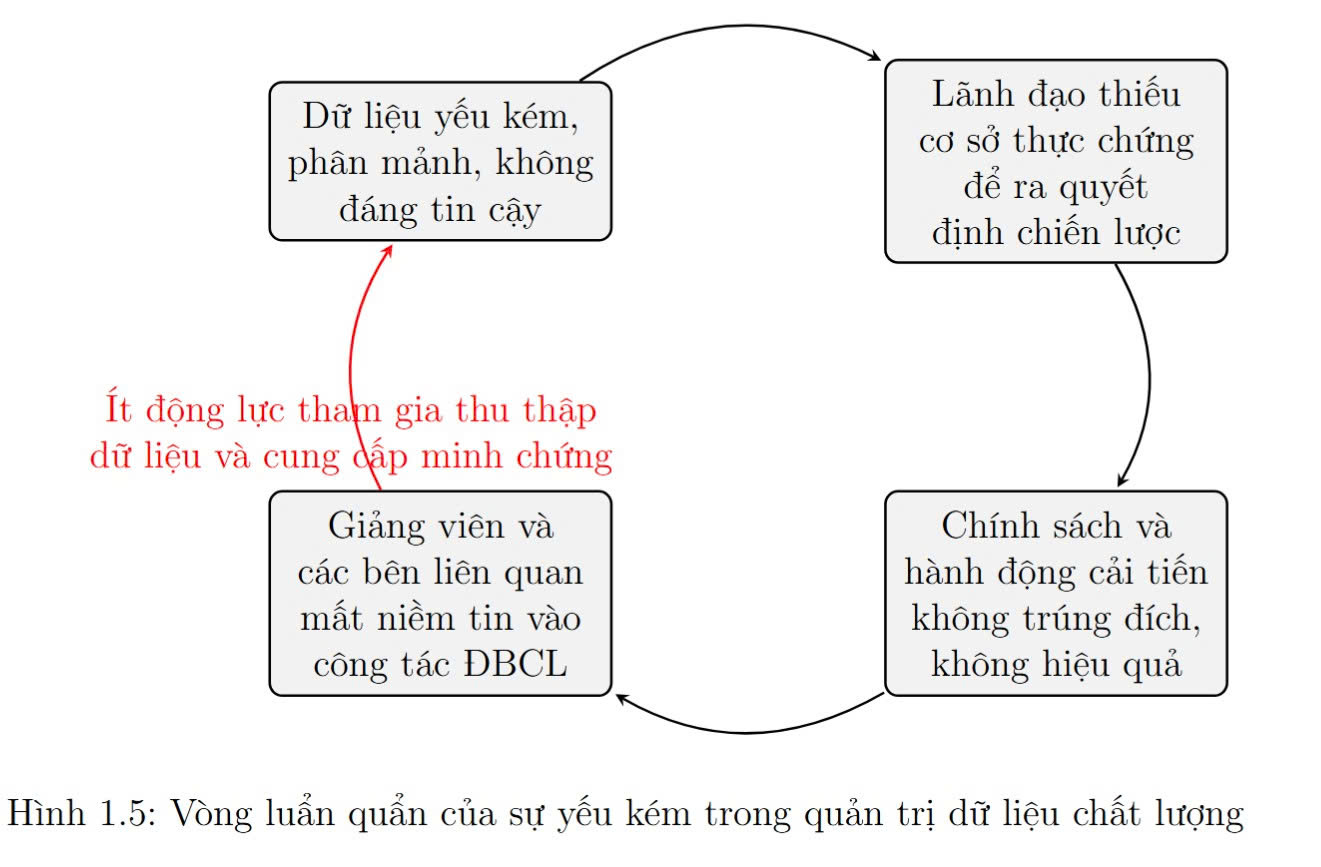
\includegraphics[width=\textwidth]{image/vong_lan_quan_trong_quan_tri_du_lieu_gd.jpg}
\caption{质量数据管理薄弱的恶性循环}
\label{fig:vong_luan_quan}
\end{figure}

这个循环自我强化,并将系统抑制在一种停滞状态。它始于\textbf{数据薄弱},导致\textbf{领导层缺乏实证依据}进行战略决策。当没有数据时,领导者被迫依赖经验和直觉进行管理,使得\textbf{改进政策和行动不具针对性}、效率低下。这导致\textbf{教师及利益相关者对质量保障工作的价值失去信心},视其为无益的行政活动。一旦失去信心,他们将\textbf{缺乏认真参与数据收集和提供证据的动力},循环回到起点,进一步加固了数据持续薄弱的状况。

打破这个恶性循环需要一场革命性的投资,一次对技术(构建集成的质量保障管理信息系统)和人(提升数据分析能力和形成基于证据的管理文化)的同步"推动"。这是最大的挑战,但也是开启一个新发展阶段——一个质量得到实质性改进的阶段——最关键的钥匙。

% het goi 8



\section{全景图与挑战的系统性互动}
\label{sec:buc_tranh_tong_hop}

通过V-AQA模型五个要素的详细分析,已阐明了越南高等教育质量保障体系中的具体"瓶颈"。为了获得一个整体和系统的视角,下表\ref{tbl:thach_thuc_tong_hop}将总结核心挑战、已证明的实际表现及其相应的系统性原因。

\begin{longtable}{|p{0.25\textwidth}|p{0.35\textwidth}|p{0.35\textwidth}|}
    \caption{基于V-AQA模型的核心挑战总结}
    \label{tbl:thach_thuc_tong_hop} \\
    \hline
    \textbf{V-AQA要素} & \textbf{在越南的实际表现} & \textbf{系统性原因} \\
    \hline
    \endfirsthead
    
    \multicolumn{3}{c}%
    {{\bfseries \tablename\ \thetable{} -- 续前页}} \\
    \hline
    \textbf{V-AQA要素} & \textbf{在越南的实际表现} & \textbf{系统性原因} \\
    \hline
    \endhead

    \hline \multicolumn{3}{r}{{\textit{续下页}}} \\
    \endfoot

    \hline
    \endlastfoot

    % 表格数据
    \textbf{1. 领导与治理} &
    推动自主的政策与合规性管理实践之间的矛盾;领导角色被限制在满足行政要求,而非进行质量战略治理。 &
    "主管部门"机制依然存在,削弱了校董会的实质性自主权;自主的法律框架不完善;来自上级的合规压力。 \\
    \hline
    
    \textbf{2. 质量文化} &
    对质量的认识仍具"反应性"和形式化;缺乏来自内部的持续改进文化。(证据:通过入学率反映的信任波动\footcite{hutech_khao_sat_2022};需要像HUTECH案例那样的强力促进机制)。 &
    自上而下的集中式治理体系;缺乏实质性自主权;缺乏针对团队的关于质量管理和质量文化的系统培训项目。 \\
    \hline
    
    \textbf{3. 利益相关者的参与} &
    缺乏从企业收集实质性反馈的机制;参与仅停留在"咨询"、"形式化"层面;实际合作比例非常低(根据世界银行数据低于3\%\footcite{worldbank_improvingperformance_2020})。 &
    封闭式管理文化,"象牙塔"思维;缺乏鼓励合作的机制;未能广泛建立互利共赢的双边合作模式。 \\
    \hline
    
    \textbf{4. 内部流程} &
    培养方案设计模糊,与实践脱节,打破了"建设性对齐"原则\footcite{Biggs2011};物质设施(特别是信息通信技术)落后;数据系统("阿喀琉斯之踵")薄弱、碎片化\footcite{worldbank_improvingperformance_2020}。 &
    传统的、重理论的培养方案设计思维;投资预算有限;官僚化的采购流程;缺乏集成的管理信息系统(HEMIS, QA-MIS)。 \\
    \hline
    
    \textbf{5. 合作与协调} &
    内部各处、室、院系之间的"孤岛"状态;各校之间的竞争环境压倒了合作与分享精神;与社会的联系松散,缺乏战略。 &
    "本位主义"、"部门主义"思维;缺乏实质性的标杆比对和相互学习机制;缺乏建立和维持战略伙伴关系的能力。 \\
    \hline
\end{longtable}

\subsection{挑战的互动与恶性循环}
\label{subsec:vong_lap_luan_quan}

将表\ref{tbl:thach_thuc_tong_hop}中的挑战系统化后,揭示了一个重要事实:它们并非独立存在。相反,它们具有因果关系,相互作用并相互强化,形成了抑制整个体系发展的\textbf{"恶性循环"}。识别这些循环是理解为何零散、片面的解决方案(例如:只专注于培训如何编写预期学习成果,或只投资购买设备)通常无法带来可持续效果的关键。基于本章的全部分析,可以为越南高等教育中运行的一个典型循环建模如下:

\begin{enumerate}
    \item \textbf{停滞的起点:} 循环始于\textbf{要素一——领导与治理},在此,领导者被困在自主政策和带有浓厚合规性的管理实践之间。来自"主管部门"的压力和复杂的行政规定迫使他们优先完成报告和应付上级要求,而不是专注于长期的质量战略\footcite{lypham_aosat_2024}。

    \item \textbf{"滋养"应付文化:} 当领导层只关注合规时,他们无法激励和建立一个主动改进的\textbf{要素二——质量文化}。取而代之的是,一种"反应性"和被动的文化将继续占主导地位,教师和员工将质量保障活动视为一项无益的行政负担\footcite{vjol_reactiveculture_2021}。
    
    \item \textbf{对外部世界关上大门:} 在一个缺乏改进动力、只关注内部合规问题的文化环境中,与外部各方的\textbf{合作与协调(要素五)}不被视为战略优先。学校缺乏动力和能力去主动构建像行业咨询委员会这样的实质性合作模式\footcite{buildit_iab_impact}。
    
    \item \textbf{加剧与市场的差距:} 当合作松散时,\textbf{利益相关者的参与(要素三)}仅停留在形式层面。培养方案无法从雇主那里获得有价值的反馈。这直接导致\textbf{内部流程(要素四)},特别是培养方案设计环节,变得陈旧,无法满足市场需求,造成产出质量低下,并加剧了"技能差距"\footcite{britishcouncil_skills_gap_2021}。
    
    \item \textbf{巩固数据薄弱环节:} 产出质量低下以及与企业联系不紧密,使得收集关于学生就业、雇主满意度的数据变得困难。这使得体系的"阿喀琉斯之踵"——\textbf{数据系统的薄弱(要素四的一部分)}——日益严重\footcite{worldbank_improvingperformance_2020}。
    
    \item \textbf{循环闭合:} 最后,数据的薄弱反过来又巩固了循环的起点。它使得\textbf{领导者更加缺乏实证依据}来做决策,导致他们更倾向于沿用旧的管理方式,依赖经验和行政命令。恶性循环就这样自我巩固,并将系统抑制在一种停滞状态。
\end{enumerate}

这个已被国际专家在分析发展中国家质量保障体系时警示过的恶性循环\footcite{aunsec_redesigningIQA_2022},揭示了一个现实:如果不改善与企业的联系,就无法解决预期学习成果的问题;而如果管理文化仍然封闭,领导层缺乏决策数据,也无法改善这种联系。因此,任何干预方案都需要采取一种系统性的方法,同时作用于问题的多个要素,而不是只关注一个表面的症状。

% het goi 9 chuong 3



\section*{第三章结论:体系诊断与改革模型的紧迫性}
\addcontentsline{toc}{section}{第三章结论}

第三章已完成其核心任务,即"解剖"越南高等教育外部质量保障体系的现状,特别是在2015-2024年阶段。通过结合宏观数据分析、国际报告、深入研究和实践案例研究,本章提供了一幅全景、多维度的画面,描绘了越南高等教育所面临的系统性挑战。本章的核心论点——即在规模增长与产出质量之间存在一个\textbf{"发展悖论"}\footcite{aunsec_redesigningIQA_2022}——已得到了一致且有说服力的证明。

本章的分析表明,在学生规模和办学机构数量增长的亮眼数字背后,是一个充满质量挑战的现实。规模增长曲线与学生就业率下降曲线之间日益扩大的分化,已将这一悖论可视化。企业面临的严重技能差距,以及毕业生失业或从事与专业不符工作的状况,是培养与社会需求"脱节"的无可辩驳的证据。

通过V-AQA模型的视角,本章深入解释了上述悖论的根本原因,证明了存在五个相互紧密关联的核心挑战群:
\begin{enumerate}
    \item \textbf{关于领导与治理:} 推动自主的政策与仍然带有浓厚合规性的管理实践之间的矛盾,限制了领导者的战略角色,迫使他们优先处理行政活动而非长期的质量改进战略。
    
    \item \textbf{关于质量文化:} 上述治理模式的直接后果是,"反应型"和应付式的"质量文化"占据主导地位,在此文化中,质量保障活动被视为一种行政负担,而非内在的改进动力。
    
    \item \textbf{关于利益相关者的参与:} 与劳动力市场日益扩大的差距以及与企业界缺乏实质性联系,导致培养方案变得陈旧且缺乏实践性。
    
    \item \textbf{关于内部流程:} 在培养方案设计、物质设施投资,特别是被视为体系"阿喀琉斯之踵"的数据管理系统薄弱等方面的严重瓶颈,瘫痪了基于证据进行决策的能力。
    
    \item \textbf{关于合作与协调:} 校内各单位之间、各校之间以及学校与社会之间的"孤岛"状态和碎片化,削弱了整个体系的协同力量和学习能力。
\end{enumerate}

更重要的是,本章指出这些挑战并非孤立存在。它们相互交织、相互强化,形成了抑制整个体系发展的\textbf{"恶性循环"}\footcite{aunsec_redesigningIQA_2022}。数据管理的薄弱削弱了领导能力,从而侵蚀了质量文化并阻碍了合作努力。这个循环解释了为何过去许多零散、片面的改革努力通常无法带来可持续的效果。它申明,如果不改善与企业的联系,就无法解决预期学习成果的问题;而如果管理文化仍然封闭,领导层缺乏决策数据,也无法改善这种联系。

通过对越南高等教育质量保障体系的"病症"进行全面和系统的"诊断",本章提供了一个坚实的实践基础,申明了全面改革模型的迫切需要。分析不仅止于指出薄弱环节,还通过对胡志明市技术大学、BUILD-IT联盟或VinUni大学的案例研究,启示了潜在的方向和解决方案。基于这一已深入分析的实践基础,下一章将承担起提出战略性解决方案和具体路线图的任务,以构建和实施\textbf{越南适应性质量保障模型(V-AQA)},旨在逐步解开已识别的症结,打破恶性循环,并使越南高等教育质量保障体系趋近区域和国际标准。

% het goi 10 chuong 3





















